% shared preamble of the theory figures (white background, purple / black theme, sans-serif)
\documentclass[tikz,border=8pt]{standalone}
\usepackage[T1]{fontenc}
\usepackage[scaled=0.92]{helvet}
\renewcommand{\familydefault}{\sfdefault}
\usepackage{amsmath,amssymb}
\usepackage[helvet]{sfmath}
\usetikzlibrary{arrows.meta,calc,decorations.pathreplacing,positioning,backgrounds}
\definecolor{ink}{HTML}{1A1A1F}
\definecolor{cohesin}{HTML}{6A3DE8}
\definecolor{condensin}{HTML}{1BAF7A}
\definecolor{fwd}{HTML}{D1303F}      % CTCF pointing right
\definecolor{rev}{HTML}{2B62D9}      % CTCF pointing left
\definecolor{panel}{HTML}{F8F6FD}
\definecolor{panelline}{HTML}{E3DDF5}
\tikzset{
  fiber/.style={line width=2.1pt,ink,line cap=round,line join=round},
  halo/.style={line width=6pt,white,line cap=round},
  lab/.style={font=\small,text=ink},
  note/.style={font=\footnotesize,text=ink!60},
  hd/.style={font=\bfseries\small,text=ink,anchor=west},
  leader/.style={line width=0.6pt,ink!45},
}
% soft panel, numbered badge, heading
\newcommand{\panelbg}[4]{\draw[rounded corners=9pt,fill=panel,draw=panelline,line width=0.9pt] (#1,#2) rectangle (#3,#4);}
\newcommand{\badge}[3]{\fill[ink] (#1,#2) circle (0.21);\node[white,font=\bfseries\footnotesize] at (#1,#2) {#3};}
% CTCF: a protein on the fibre carrying an arrow that gives the motif direction (f = right, r = left)
\newcommand{\protf}[2]{\draw[rounded corners=3.5pt,line width=0.6pt,draw=fwd!65!black,fill=fwd] (#1-0.3,#2-0.19) rectangle (#1+0.3,#2+0.19);
  \draw[white,line width=1.5pt,-{Stealth[length=3.4pt,width=4.4pt]}] (#1-0.15,#2)--(#1+0.16,#2);}
\newcommand{\protr}[2]{\draw[rounded corners=3.5pt,line width=0.6pt,draw=rev!65!black,fill=rev] (#1-0.3,#2-0.19) rectangle (#1+0.3,#2+0.19);
  \draw[white,line width=1.5pt,-{Stealth[length=3.4pt,width=4.4pt]}] (#1+0.15,#2)--(#1-0.16,#2);}
\newcommand{\prot}[3]{\csname prot#3\endcsname{#1}{#2}}
% ring seen at an angle, drawn as a tube (dark outline, light core); back half and front half
\newcommand{\ringpart}[5]{\draw[line width=4.6pt,#3!80!black,line cap=round] ([shift={(#1,#2)}]#4:0.55 and 0.21) arc[start angle=#4,end angle=#5,x radius=0.55,y radius=0.21];
  \draw[line width=2.4pt,#3!55!white,line cap=round] ([shift={(#1,#2)}]#4:0.55 and 0.21) arc[start angle=#4,end angle=#5,x radius=0.55,y radius=0.21];}
\newcommand{\ringback}[3]{\ringpart{#1}{#2}{#3}{180}{0}}
\newcommand{\ringfront}[3]{\ringpart{#1}{#2}{#3}{180}{360}}
% smooth loop whose foot (ring) is at (cx,y0): half-width W, height H, ring colour
\newcommand{\lloop}[5]{%
  \ringback{#1}{#2}{#5}%
  \draw[fiber] (#1-0.3,#2) .. controls (#1-0.3,#2+0.25*#4) and (#1-#3,#2+0.2*#4) .. (#1-#3,#2+0.55*#4)
     .. controls (#1-#3,#2+0.95*#4) and (#1-0.5*#3,#2+#4) .. (#1,#2+#4)
     .. controls (#1+0.5*#3,#2+#4) and (#1+#3,#2+0.95*#4) .. (#1+#3,#2+0.55*#4)
     .. controls (#1+#3,#2+0.2*#4) and (#1+0.3,#2+0.25*#4) .. (#1+0.3,#2);%
  \ringfront{#1}{#2}{#5}}
% gently undulating fibre from x0 to the loop foot at cx (height y0), and from x1
\newcommand{\base}[4]{%
  \draw[fiber] plot[smooth] coordinates {(#1,0.05) (#1+0.35*#3-0.35*#1,-0.05) (#3-1.4,0.04)} .. controls (#3-0.6,0.02) and (#3-0.3,0.05) .. (#3-0.3,#4);
  \draw[fiber] plot[smooth] coordinates {(#2,-0.05) (#2-0.35*#2+0.35*#3,0.05) (#3+1.4,-0.04)} .. controls (#3+0.6,-0.02) and (#3+0.3,0.05) .. (#3+0.3,#4);}
% stop sign for a blocked leg and a leg arrow
\newcommand{\stopbar}[3]{\draw[#3,line width=2.4pt,line cap=round] (#1,#2-0.2)--(#1,#2+0.2);}
\newcommand{\legarrow}[3]{\draw[cohesin,line width=1.6pt,-{Stealth[length=5pt,width=6pt]},line cap=round] (#1,#3)--(#2,#3);}

\tikzset{ln/.style={line width=0.7pt,ink!45},arc/.style={line width=1.1pt,cohesin!85},cand/.style={line width=2pt,A}}
\definecolor{L}{HTML}{6A3DE8}\definecolor{R}{HTML}{1A1A1F}\definecolor{A}{HTML}{D1303F}\definecolor{B}{HTML}{5B4FD6}
\begin{document}
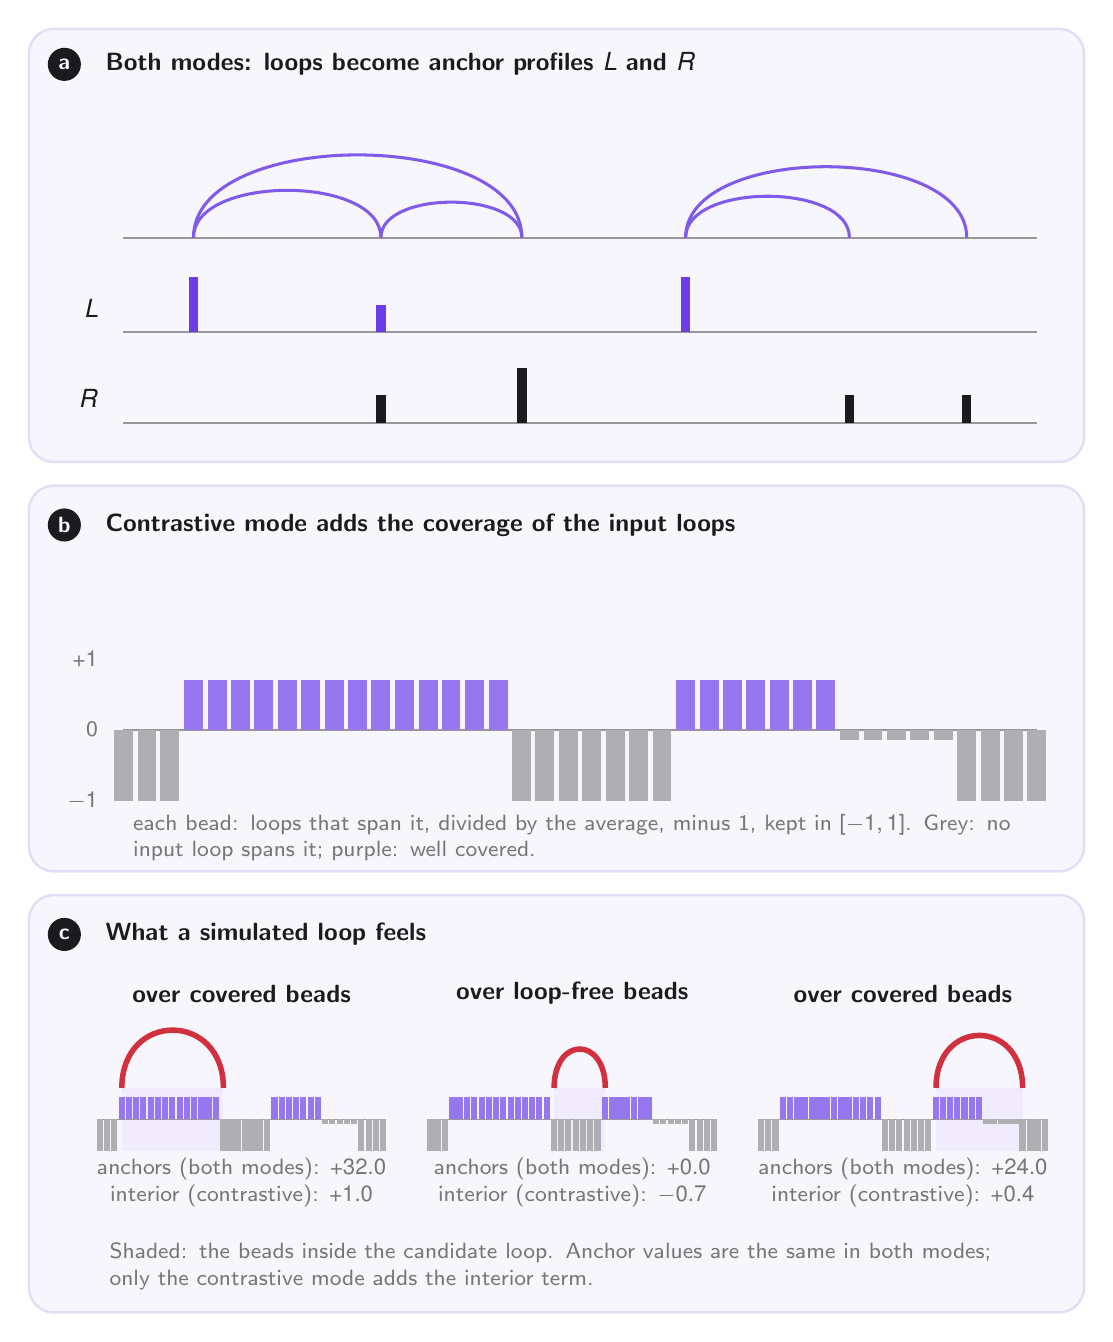
\begin{tikzpicture}
  \panelbg{0}{-0.2}{13.4}{5.3}\panelbg{0}{-5.4}{13.4}{-0.5}\panelbg{0}{-11.0}{13.4}{-5.7}
  \badge{0.45}{4.85}{a}\node[hd] at (0.85,4.85) {Both modes: loops become anchor profiles $L$ and $R$};
  \badge{0.45}{-1.0}{b}\node[hd] at (0.85,-1.0) {Contrastive mode adds the coverage of the input loops};
  \badge{0.45}{-6.2}{c}\node[hd] at (0.85,-6.2) {What a simulated loop feels};
  \draw[ln] (1.20,2.65)--(12.80,2.65);
  \draw[arc] (2.09,2.65) .. controls (2.09,3.45) and (4.47,3.45) .. (4.47,2.65);
  \draw[arc] (2.09,2.65) .. controls (2.09,4.05) and (6.26,4.05) .. (6.26,2.65);
  \draw[arc] (4.47,2.65) .. controls (4.47,3.25) and (6.26,3.25) .. (6.26,2.65);
  \draw[arc] (8.34,2.65) .. controls (8.34,3.85) and (11.91,3.85) .. (11.91,2.65);
  \draw[arc] (8.34,2.65) .. controls (8.34,3.35) and (10.42,3.35) .. (10.42,2.65);
  \draw[ln] (1.20,1.45)--(12.80,1.45);\node[lab,anchor=east] at (1.0,1.75) {$L$};
  \fill[L] (2.03,1.45) rectangle (2.15,2.15);
  \fill[L] (4.41,1.45) rectangle (4.53,1.80);
  \fill[L] (8.28,1.45) rectangle (8.40,2.15);
  \draw[ln] (1.20,0.3)--(12.80,0.3);\node[lab,anchor=east] at (1.0,0.6) {$R$};
  \fill[R] (4.41,0.3) rectangle (4.53,0.65);
  \fill[R] (6.20,0.3) rectangle (6.32,1.00);
  \fill[R] (10.36,0.3) rectangle (10.48,0.65);
  \fill[R] (11.85,0.3) rectangle (11.97,0.65);
  \draw[ln] (1.20,-3.6)--(12.80,-3.6);
  \node[note,anchor=east] at (1.0,-2.7) {$+1$};\node[note,anchor=east] at (1.0,-4.5) {$-1$};\node[note,anchor=east] at (1.0,-3.6) {0};
  \fill[ink!35] (1.08,-3.6) rectangle (1.32,-4.50);
  \fill[ink!35] (1.38,-3.6) rectangle (1.62,-4.50);
  \fill[ink!35] (1.67,-3.6) rectangle (1.91,-4.50);
  \fill[L!70] (1.97,-3.6) rectangle (2.21,-2.97);
  \fill[L!70] (2.27,-3.6) rectangle (2.51,-2.97);
  \fill[L!70] (2.57,-3.6) rectangle (2.81,-2.97);
  \fill[L!70] (2.86,-3.6) rectangle (3.10,-2.97);
  \fill[L!70] (3.16,-3.6) rectangle (3.40,-2.97);
  \fill[L!70] (3.46,-3.6) rectangle (3.70,-2.97);
  \fill[L!70] (3.76,-3.6) rectangle (4.00,-2.97);
  \fill[L!70] (4.05,-3.6) rectangle (4.29,-2.97);
  \fill[L!70] (4.35,-3.6) rectangle (4.59,-2.97);
  \fill[L!70] (4.65,-3.6) rectangle (4.89,-2.97);
  \fill[L!70] (4.95,-3.6) rectangle (5.19,-2.97);
  \fill[L!70] (5.24,-3.6) rectangle (5.48,-2.97);
  \fill[L!70] (5.54,-3.6) rectangle (5.78,-2.97);
  \fill[L!70] (5.84,-3.6) rectangle (6.08,-2.97);
  \fill[ink!35] (6.14,-3.6) rectangle (6.38,-4.50);
  \fill[ink!35] (6.43,-3.6) rectangle (6.67,-4.50);
  \fill[ink!35] (6.73,-3.6) rectangle (6.97,-4.50);
  \fill[ink!35] (7.03,-3.6) rectangle (7.27,-4.50);
  \fill[ink!35] (7.33,-3.6) rectangle (7.57,-4.50);
  \fill[ink!35] (7.62,-3.6) rectangle (7.86,-4.50);
  \fill[ink!35] (7.92,-3.6) rectangle (8.16,-4.50);
  \fill[L!70] (8.22,-3.6) rectangle (8.46,-2.97);
  \fill[L!70] (8.52,-3.6) rectangle (8.76,-2.97);
  \fill[L!70] (8.81,-3.6) rectangle (9.05,-2.97);
  \fill[L!70] (9.11,-3.6) rectangle (9.35,-2.97);
  \fill[L!70] (9.41,-3.6) rectangle (9.65,-2.97);
  \fill[L!70] (9.71,-3.6) rectangle (9.95,-2.97);
  \fill[L!70] (10.00,-3.6) rectangle (10.24,-2.97);
  \fill[ink!35] (10.30,-3.6) rectangle (10.54,-3.73);
  \fill[ink!35] (10.60,-3.6) rectangle (10.84,-3.73);
  \fill[ink!35] (10.90,-3.6) rectangle (11.14,-3.73);
  \fill[ink!35] (11.19,-3.6) rectangle (11.43,-3.73);
  \fill[ink!35] (11.49,-3.6) rectangle (11.73,-3.73);
  \fill[ink!35] (11.79,-3.6) rectangle (12.03,-4.50);
  \fill[ink!35] (12.09,-3.6) rectangle (12.33,-4.50);
  \fill[ink!35] (12.38,-3.6) rectangle (12.62,-4.50);
  \fill[ink!35] (12.68,-3.6) rectangle (12.92,-4.50);
  \node[note,text width=11.4cm,anchor=north west] at (1.2,-4.55) {each bead: loops that span it, divided by the average, minus 1, kept in $[-1,1]$. Grey: no input loop spans it; purple: well covered.};
  \fill[L!10] (1.18,-8.950000000000001) rectangle (2.47,-8.15);
  \draw[ln] (0.90,-8.55)--(4.50,-8.55);
  \fill[ink!35] (0.86,-8.55) rectangle (0.94,-8.95);
  \fill[ink!35] (0.95,-8.55) rectangle (1.03,-8.95);
  \fill[ink!35] (1.04,-8.55) rectangle (1.12,-8.95);
  \fill[L!70] (1.14,-8.55) rectangle (1.22,-8.27);
  \fill[L!70] (1.23,-8.55) rectangle (1.31,-8.27);
  \fill[L!70] (1.32,-8.55) rectangle (1.40,-8.27);
  \fill[L!70] (1.41,-8.55) rectangle (1.49,-8.27);
  \fill[L!70] (1.51,-8.55) rectangle (1.59,-8.27);
  \fill[L!70] (1.60,-8.55) rectangle (1.68,-8.27);
  \fill[L!70] (1.69,-8.55) rectangle (1.77,-8.27);
  \fill[L!70] (1.78,-8.55) rectangle (1.86,-8.27);
  \fill[L!70] (1.88,-8.55) rectangle (1.96,-8.27);
  \fill[L!70] (1.97,-8.55) rectangle (2.05,-8.27);
  \fill[L!70] (2.06,-8.55) rectangle (2.14,-8.27);
  \fill[L!70] (2.15,-8.55) rectangle (2.23,-8.27);
  \fill[L!70] (2.24,-8.55) rectangle (2.32,-8.27);
  \fill[L!70] (2.34,-8.55) rectangle (2.42,-8.27);
  \fill[ink!35] (2.43,-8.55) rectangle (2.51,-8.95);
  \fill[ink!35] (2.52,-8.55) rectangle (2.60,-8.95);
  \fill[ink!35] (2.61,-8.55) rectangle (2.69,-8.95);
  \fill[ink!35] (2.71,-8.55) rectangle (2.79,-8.95);
  \fill[ink!35] (2.80,-8.55) rectangle (2.88,-8.95);
  \fill[ink!35] (2.89,-8.55) rectangle (2.97,-8.95);
  \fill[ink!35] (2.98,-8.55) rectangle (3.06,-8.95);
  \fill[L!70] (3.08,-8.55) rectangle (3.16,-8.27);
  \fill[L!70] (3.17,-8.55) rectangle (3.25,-8.27);
  \fill[L!70] (3.26,-8.55) rectangle (3.34,-8.27);
  \fill[L!70] (3.35,-8.55) rectangle (3.43,-8.27);
  \fill[L!70] (3.44,-8.55) rectangle (3.52,-8.27);
  \fill[L!70] (3.54,-8.55) rectangle (3.62,-8.27);
  \fill[L!70] (3.63,-8.55) rectangle (3.71,-8.27);
  \fill[ink!35] (3.72,-8.55) rectangle (3.80,-8.61);
  \fill[ink!35] (3.81,-8.55) rectangle (3.89,-8.61);
  \fill[ink!35] (3.91,-8.55) rectangle (3.99,-8.61);
  \fill[ink!35] (4.00,-8.55) rectangle (4.08,-8.61);
  \fill[ink!35] (4.09,-8.55) rectangle (4.17,-8.61);
  \fill[ink!35] (4.18,-8.55) rectangle (4.26,-8.95);
  \fill[ink!35] (4.28,-8.55) rectangle (4.36,-8.95);
  \fill[ink!35] (4.37,-8.55) rectangle (4.45,-8.95);
  \fill[ink!35] (4.46,-8.55) rectangle (4.54,-8.95);
  \draw[cand] (1.18,-8.15) .. controls (1.18,-7.17) and (2.47,-7.17) .. (2.47,-8.15);
  \node[lab] at (2.70,-6.95) {\bfseries over covered beads};
  \node[note,align=center] at (2.70,-9.35) {anchors (both modes): $+32.0$\\interior (contrastive): $+1.0$};
  \fill[L!10] (6.67,-8.950000000000001) rectangle (7.32,-8.15);
  \draw[ln] (5.10,-8.55)--(8.70,-8.55);
  \fill[ink!35] (5.06,-8.55) rectangle (5.14,-8.95);
  \fill[ink!35] (5.15,-8.55) rectangle (5.23,-8.95);
  \fill[ink!35] (5.24,-8.55) rectangle (5.32,-8.95);
  \fill[L!70] (5.34,-8.55) rectangle (5.42,-8.27);
  \fill[L!70] (5.43,-8.55) rectangle (5.51,-8.27);
  \fill[L!70] (5.52,-8.55) rectangle (5.60,-8.27);
  \fill[L!70] (5.61,-8.55) rectangle (5.69,-8.27);
  \fill[L!70] (5.71,-8.55) rectangle (5.79,-8.27);
  \fill[L!70] (5.80,-8.55) rectangle (5.88,-8.27);
  \fill[L!70] (5.89,-8.55) rectangle (5.97,-8.27);
  \fill[L!70] (5.98,-8.55) rectangle (6.06,-8.27);
  \fill[L!70] (6.08,-8.55) rectangle (6.16,-8.27);
  \fill[L!70] (6.17,-8.55) rectangle (6.25,-8.27);
  \fill[L!70] (6.26,-8.55) rectangle (6.34,-8.27);
  \fill[L!70] (6.35,-8.55) rectangle (6.43,-8.27);
  \fill[L!70] (6.44,-8.55) rectangle (6.52,-8.27);
  \fill[L!70] (6.54,-8.55) rectangle (6.62,-8.27);
  \fill[ink!35] (6.63,-8.55) rectangle (6.71,-8.95);
  \fill[ink!35] (6.72,-8.55) rectangle (6.80,-8.95);
  \fill[ink!35] (6.81,-8.55) rectangle (6.89,-8.95);
  \fill[ink!35] (6.91,-8.55) rectangle (6.99,-8.95);
  \fill[ink!35] (7.00,-8.55) rectangle (7.08,-8.95);
  \fill[ink!35] (7.09,-8.55) rectangle (7.17,-8.95);
  \fill[ink!35] (7.18,-8.55) rectangle (7.26,-8.95);
  \fill[L!70] (7.28,-8.55) rectangle (7.36,-8.27);
  \fill[L!70] (7.37,-8.55) rectangle (7.45,-8.27);
  \fill[L!70] (7.46,-8.55) rectangle (7.54,-8.27);
  \fill[L!70] (7.55,-8.55) rectangle (7.63,-8.27);
  \fill[L!70] (7.64,-8.55) rectangle (7.72,-8.27);
  \fill[L!70] (7.74,-8.55) rectangle (7.82,-8.27);
  \fill[L!70] (7.83,-8.55) rectangle (7.91,-8.27);
  \fill[ink!35] (7.92,-8.55) rectangle (8.00,-8.61);
  \fill[ink!35] (8.01,-8.55) rectangle (8.09,-8.61);
  \fill[ink!35] (8.11,-8.55) rectangle (8.19,-8.61);
  \fill[ink!35] (8.20,-8.55) rectangle (8.28,-8.61);
  \fill[ink!35] (8.29,-8.55) rectangle (8.37,-8.61);
  \fill[ink!35] (8.38,-8.55) rectangle (8.46,-8.95);
  \fill[ink!35] (8.48,-8.55) rectangle (8.56,-8.95);
  \fill[ink!35] (8.57,-8.55) rectangle (8.65,-8.95);
  \fill[ink!35] (8.66,-8.55) rectangle (8.74,-8.95);
  \draw[cand] (6.67,-8.15) .. controls (6.67,-7.49) and (7.32,-7.49) .. (7.32,-8.15);
  \node[lab] at (6.90,-6.95) {\bfseries over loop-free beads};
  \node[note,align=center] at (6.90,-9.35) {anchors (both modes): $+0.0$\\interior (contrastive): $-0.7$};
  \fill[L!10] (11.52,-8.950000000000001) rectangle (12.62,-8.15);
  \draw[ln] (9.30,-8.55)--(12.90,-8.55);
  \fill[ink!35] (9.26,-8.55) rectangle (9.34,-8.95);
  \fill[ink!35] (9.35,-8.55) rectangle (9.43,-8.95);
  \fill[ink!35] (9.44,-8.55) rectangle (9.52,-8.95);
  \fill[L!70] (9.54,-8.55) rectangle (9.62,-8.27);
  \fill[L!70] (9.63,-8.55) rectangle (9.71,-8.27);
  \fill[L!70] (9.72,-8.55) rectangle (9.80,-8.27);
  \fill[L!70] (9.81,-8.55) rectangle (9.89,-8.27);
  \fill[L!70] (9.91,-8.55) rectangle (9.99,-8.27);
  \fill[L!70] (10.00,-8.55) rectangle (10.08,-8.27);
  \fill[L!70] (10.09,-8.55) rectangle (10.17,-8.27);
  \fill[L!70] (10.18,-8.55) rectangle (10.26,-8.27);
  \fill[L!70] (10.28,-8.55) rectangle (10.36,-8.27);
  \fill[L!70] (10.37,-8.55) rectangle (10.45,-8.27);
  \fill[L!70] (10.46,-8.55) rectangle (10.54,-8.27);
  \fill[L!70] (10.55,-8.55) rectangle (10.63,-8.27);
  \fill[L!70] (10.64,-8.55) rectangle (10.72,-8.27);
  \fill[L!70] (10.74,-8.55) rectangle (10.82,-8.27);
  \fill[ink!35] (10.83,-8.55) rectangle (10.91,-8.95);
  \fill[ink!35] (10.92,-8.55) rectangle (11.00,-8.95);
  \fill[ink!35] (11.01,-8.55) rectangle (11.09,-8.95);
  \fill[ink!35] (11.11,-8.55) rectangle (11.19,-8.95);
  \fill[ink!35] (11.20,-8.55) rectangle (11.28,-8.95);
  \fill[ink!35] (11.29,-8.55) rectangle (11.37,-8.95);
  \fill[ink!35] (11.38,-8.55) rectangle (11.46,-8.95);
  \fill[L!70] (11.48,-8.55) rectangle (11.56,-8.27);
  \fill[L!70] (11.57,-8.55) rectangle (11.65,-8.27);
  \fill[L!70] (11.66,-8.55) rectangle (11.74,-8.27);
  \fill[L!70] (11.75,-8.55) rectangle (11.83,-8.27);
  \fill[L!70] (11.84,-8.55) rectangle (11.92,-8.27);
  \fill[L!70] (11.94,-8.55) rectangle (12.02,-8.27);
  \fill[L!70] (12.03,-8.55) rectangle (12.11,-8.27);
  \fill[ink!35] (12.12,-8.55) rectangle (12.20,-8.61);
  \fill[ink!35] (12.21,-8.55) rectangle (12.29,-8.61);
  \fill[ink!35] (12.31,-8.55) rectangle (12.39,-8.61);
  \fill[ink!35] (12.40,-8.55) rectangle (12.48,-8.61);
  \fill[ink!35] (12.49,-8.55) rectangle (12.57,-8.61);
  \fill[ink!35] (12.58,-8.55) rectangle (12.66,-8.95);
  \fill[ink!35] (12.68,-8.55) rectangle (12.76,-8.95);
  \fill[ink!35] (12.77,-8.55) rectangle (12.85,-8.95);
  \fill[ink!35] (12.86,-8.55) rectangle (12.94,-8.95);
  \draw[cand] (11.52,-8.15) .. controls (11.52,-7.26) and (12.62,-7.26) .. (12.62,-8.15);
  \node[lab] at (11.10,-6.95) {\bfseries over covered beads};
  \node[note,align=center] at (11.10,-9.35) {anchors (both modes): $+24.0$\\interior (contrastive): $+0.4$};
  \node[note,text width=11.8cm,anchor=north west] at (0.9,-10.0) {Shaded: the beads inside the candidate loop. Anchor values are the same in both modes; only the contrastive mode adds the interior term.};
\end{tikzpicture}
\end{document}
